\section{Contrastive Fine-Tuning as a Probe}
\label{contrastive}


BFT shows what happens when reverse supervision is made explicit. Contrastive
fine-tuning poses a different question. Can reverse capability be recovered
without reverse labels, provided the training objective preserves semantic
proximity between original and obfuscated programs? We treat CFT as a mechanistic
probe, not as a production recipe. If directional capability loss has a
representational component, then a forward-only objective augmented with semantic
contrast should reduce that component on at least the simpler inverses.



CFT adds a contrastive objective to the forward generation loss. Each training
example contains an anchor program, its obfuscated counterpart as a positive
example, and an unrelated program as a negative example, see Figure~\ref{fig:contrastive_prompting}. The model is optimized
to generate the forward transformation while distinguishing semantically related
from unrelated pairs. Following prior contrastive learning formulations~\cite{chen2020simple,
he2020momentum},~\cite{jain2021contracode, li2022coderetriever} the combined loss is

\begin{equation}
\mathcal{L}_{\text{CFT}} = \lambda_1 \mathcal{L}_{\text{gen}} + \lambda_2(\mathcal{L}_{\text{pos}} + \mathcal{L}_{\text{neg}}),
\end{equation}

with $\lambda_1 = \lambda_2 = 1$ in our open-source runs. The salient property of
this objective is that CFT never observes a reverse label. Any recovery in the
reverse direction must therefore arise from preserving semantic structure while
the model learns the forward transformation.

% \begin{figure*}[!ht]
%     \centering
%     \begin{tikzpicture}[scale=0.9, every node/.style={scale=0.9}]
%         \definecolor{poscolor}{RGB}{0,158,115}
%         \definecolor{negcolor}{RGB}{213,94,0}
%         \definecolor{gencolor}{RGB}{86,180,233}
%         \definecolor{codebg}{RGB}{250,250,250}
%         \definecolor{textgray}{gray}{0.15}

%         % Positive Classification
%         \node[draw, fill=poscolor!20, text width=5cm, align=center, font=\small\bfseries, rounded corners=2pt]
%             at (-7, 6.2) {Positive Classification ($a$, $p$)};
%         \node[draw, fill=codebg, text width=5.8cm, align=left, font=\scriptsize, rounded corners=2pt]
%             at (-7, 4.5) {
%             \textbf{User:} Are these code snippets semantically equivalent?\\
%             Code 1: \texttt{[Anchor]}\\
%             Code 2: \texttt{[Positive]}\\
%             \textbf{Assistant:} Yes, they are equivalent...
%         };

%         % Negative Classification
%         \node[draw, fill=negcolor!20, text width=5.8cm, align=center, font=\small\bfseries, rounded corners=2pt]
%             at (0, 6.2) {Negative Classification ($a$, $n$)};
%         \node[draw, fill=codebg, text width=5.8cm, align=left, font=\scriptsize, rounded corners=2pt]
%             at (0, 4.5) {
%             \textbf{User:} Are these code snippets semantically equivalent?\\
%             Code 1: \texttt{[Anchor]}\\
%             Code 2: \texttt{[Negative]}\\
%             \textbf{Assistant:} No, they differ functionally...
%         };

%         % Forward Generation
%         \node[draw, fill=gencolor!20, text width=5.8cm, align=center, font=\small\bfseries, rounded corners=2pt]
%             at (7, 6.2) {Obfuscation Task ($a \rightarrow p$)};
%         \node[draw, fill=codebg, text width=5.8cm, align=left, font=\scriptsize, rounded corners=2pt]
%             at (7, 4.5) {
%             \textbf{User:} Obfuscate this code by \texttt{[Ofuscation Type]}...\\
%             \texttt{[Anchor]}\\
%             \textbf{Assistant:} Here's the obfuscated version:\\
%             \texttt{[Positive]}
%         };

%         % Learning Objectives
%         \draw[->, thick, poscolor] (-7, 3.4) -- (-7, 3.0);
%         \node[font=\normalsize, poscolor] at (-7, 2.8) {$\mathcal{L}_{pos}$: Minimize semantic distance};

%         \draw[->, thick, negcolor] (0, 3.4) -- (0, 3.0);
%         \node[font=\normalsize, negcolor] at (0, 2.8) {$\mathcal{L}_{neg}$: Maximize semantic distance};

%         \draw[->, thick, gencolor] (7, 3.4) -- (7, 3.0);
%         \node[font=\normalsize, gencolor] at (7, 2.8) {$\mathcal{L}_{gen}$: Learn transformation};

%         % Combined Loss
%         \node[draw, fill=white, rounded corners=3pt, text width=6cm, align=left, font=\large] 
%             at (0, 2) {$\mathcal{L}_{\text{CFT}} = \lambda_1 \mathcal{L}_{pos} + \lambda_2 \mathcal{L}_{neg} + \mathcal{L}_{gen}$};
%     \end{tikzpicture}
%     \caption{Contrastive Fine-Tuning prompting strategy.
%     %The anchor ($a$) is paired with a semantically equivalent transformation ($p$) and a dissimilar variant ($n$). The model learns to minimize semantic distance for $(a, p)$, maximize it for $(a, n)$, and generate $p$ from $a$.
%     }
%     \label{fig:contrastive_prompting}
% \end{figure*}

%%%%%%%%%%%%%%%%%%%%%%%%%%%%%%%%%%%%%%%%%%%%%%%%%%%

% \begin{figure*}[!ht]
%     \centering
%     \begin{tikzpicture}[scale=0.9, every node/.style={scale=0.9}]
%         \definecolor{poscolor}{RGB}{0,158,115}
%         \definecolor{negcolor}{RGB}{213,94,0}
%         \definecolor{gencolor}{RGB}{86,180,233}
%         \definecolor{codebg}{RGB}{250,250,250}
%         \definecolor{textgray}{gray}{0.15}

%         % Positive Classification
%         \node[draw, fill=poscolor!20, text width=5cm, align=center, font=\small\bfseries, rounded corners=2pt]
%             at (-7, 5.2) {Positive Classification ($a$, $p$)};
%         \node[draw, fill=codebg, text width=5.8cm, align=left, font=\scriptsize, rounded corners=2pt]
%             at (-7, 4.2) {
%             \textbf{User:} Are these code snippets semantically equivalent?\\
%             Code 1: \texttt{[Anchor]}\\
%             Code 2: \texttt{[Positive]}\\
%             \textbf{Assistant:} Yes, they are equivalent...
%         };

%         % Negative Classification
%         \node[draw, fill=negcolor!20, text width=5.8cm, align=center, font=\small\bfseries, rounded corners=2pt]
%             at (0, 5.2) {Negative Classification ($a$, $n$)};
%         \node[draw, fill=codebg, text width=5.8cm, align=left, font=\scriptsize, rounded corners=2pt]
%             at (0, 4.2) {
%             \textbf{User:} Are these code snippets semantically equivalent?\\
%             Code 1: \texttt{[Anchor]}\\
%             Code 2: \texttt{[Negative]}\\
%             \textbf{Assistant:} No, they differ functionally...
%         };

%         % Forward Generation
%         \node[draw, fill=gencolor!20, text width=5.8cm, align=center, font=\small\bfseries, rounded corners=2pt]
%             at (7, 5.2) {Obfuscation Task ($a \rightarrow p$)};
%         \node[draw, fill=codebg, text width=5.8cm, align=left, font=\scriptsize, rounded corners=2pt]
%             at (7, 4.2) {
%             \textbf{User:} Obfuscate this code by \texttt{[Ofuscation Type]}...\\
%             \texttt{[Anchor]}\\
%             \textbf{Assistant:} Here's the obfuscated version:\\
%             \texttt{[Positive]}
%         };

%         % Learning Objectives
%         \draw[->, thick, poscolor] (-7, 3.3) -- (-7, 3.0);
%         \node[font=\normalsize, poscolor] at (-7, 2.6) {$\mathcal{L}_{pos}$: Minimize semantic distance};

%         \draw[->, thick, negcolor] (0, 3.3) -- (0, 3.0);
%         \node[font=\normalsize, negcolor] at (0, 2.6) {$\mathcal{L}_{neg}$: Maximize semantic distance};

%         \draw[->, thick, gencolor] (7, 3.3) -- (7, 3.0);
%         \node[font=\normalsize, gencolor] at (7, 2.6) {$\mathcal{L}_{gen}$: Learn transformation};

%         % Combined Loss
%         \node[draw, fill=white, rounded corners=3pt, text width=6cm, align=left, font=\large] 
%             at (0, 1.5) {$\mathcal{L}_{\text{CFT}} = \lambda_1 \mathcal{L}_{pos} + \lambda_2 \mathcal{L}_{neg} + \mathcal{L}_{gen}$};
%     \end{tikzpicture}
%     \caption{Contrastive Fine-Tuning prompting strategy.
%     %The anchor ($a$) is paired with a semantically equivalent transformation ($p$) and a dissimilar variant ($n$). The model learns to minimize semantic distance for $(a, p)$, maximize it for $(a, n)$, and generate $p$ from $a$.
%     }
%     \label{fig:contrastive_prompting}
% \end{figure*}

%%%%%%%%%%%%%%%%%%%%%%%%%



% \begin{figure}[!ht]
%     \centering
%     \scriptsize
%     \begin{tikzpicture}[
%         node distance=0.5cm,
%         codebox/.style={rectangle, rounded corners=3pt, draw=black!40, line width=0.8pt, 
%                         fill=white, drop shadow={opacity=0.15}, 
%                         minimum height=0.8cm, align=left},
%         arrow/.style={-{Stealth[length=2mm]}, line width=1.2pt}
%     ]
    
%     % Configure Java syntax highlighting
%     \lstset{
%         language=Java,
%         basicstyle=\ttfamily\fontsize{7}{8}\selectfont,
%         keywordstyle=\color{blue!70!black}\bfseries,
%         identifierstyle=\color{black},
%         numbers=none,
%         breaklines=true,
%         xleftmargin=3pt,
%         xrightmargin=3pt,
%         backgroundcolor=\color{gray!5},
%         frame=none,
%         escapechar=@,
%         columns=flexible
%     }
    
%     % SFT: Obfuscated Input → Verbatim Reproduction (Left)
%     \node[codebox, draw=red!50, text width=0.45\columnwidth] (sft) {
%         \textbf{\footnotesize SFT: Cognitive Specialization}\\
%         \textit{\tiny Obfuscated input reproduced verbatim}\\[2pt]
%         \begin{lstlisting}
% public class Main_2 {
%   void solve() {
%     Scanner @\colorbox{red!20}{\texttt{IlIlIllIlIlI}}@ = 
%       new Scanner(System.in);
%     int @\colorbox{red!20}{\texttt{llIlIIlIIl}}@ = 
%       @\colorbox{red!20}{\texttt{IlIlIllIlIlI}}@.nextInt();
%     for (int i = @\colorbox{red!20}{\texttt{llIlIIlIIl}}@;
%          i >= 0; --i)
%       System.out.println(i);
%   }
% }
%         \end{lstlisting}
%         \vspace{2pt}
%         \textcolor{red!70!black}{\tiny\bfseries \ding{55} AST$_{\text{synt}}$ = 0.999 (99\% identifiers retained)}
%     };
    
%     % CFT: Successful Deobfuscation (Right)
%     \node[codebox, draw=green!50!black, text width=0.45\columnwidth, right=0.5cm of sft] (cft) {
%         \textbf{\footnotesize CFT: Emergent Bidirectionality}\\
%         \textit{\tiny Semantic recovery with readable identifiers}\\[2pt]
%         \begin{lstlisting}
% public class @\colorbox{green!20}{\texttt{CountingNumbers}}@ {
%   void @\colorbox{green!20}{\texttt{countDown}}@() {
%     Scanner @\colorbox{green!20}{\texttt{scanner}}@ =
%       new Scanner(System.in);
%     int @\colorbox{green!20}{\texttt{number}}@ = 
%       @\colorbox{green!20}{\texttt{scanner}}@.nextInt();
%     for (int i = @\colorbox{green!20}{\texttt{number}}@;
%          i >= 0; --i)
%       System.out.println(i);
%   }
% }
%         \end{lstlisting}
%         \vspace{2pt}
%         \textcolor{green!60!black}{\tiny\bfseries \checkmark AST$_{\text{synt}}$ = 0.17 (83\% identifiers changed)}
%     };
    
%     \end{tikzpicture}
    
%     \caption{Cognitive Specialization vs. Emergent Bidirectionality.}
%     \label{fig:cognitive_specialization}
% \end{figure}


%%%%%%%%%%%%%%%%%%%%%%%%%%%%%%%%%%%%%%%%%%%%%%%%%%


% \begin{figure}[!ht]
%     \centering
%     \scriptsize
%     \begin{tikzpicture}[
%         node distance=0.5cm,
%         codebox/.style={rectangle, rounded corners=3pt, draw=black!40, line width=0.8pt, 
%                         fill=white, drop shadow={opacity=0.15}, 
%                         minimum height=0.8cm, align=left},
%         arrow/.style={-{Stealth[length=2mm]}, line width=1.2pt}
%     ]
    
%     % Configure Java syntax highlighting
%     \lstset{
%         language=Java,
%         basicstyle=\ttfamily\fontsize{7}{8}\selectfont,
%         keywordstyle=\color{blue!70!black}\bfseries,
%         identifierstyle=\color{black},
%         numbers=none,
%         breaklines=true,
%         xleftmargin=3pt,
%         xrightmargin=3pt,
%         backgroundcolor=\color{gray!5},
%         frame=none,
%         escapechar=@,
%         columns=flexible
%     }
    
%     % SFT: Obfuscated Input → Verbatim Reproduction (Left)
%     \node[codebox, draw=red!50, text width=0.45\columnwidth] (sft) {
%         \textbf{\footnotesize SFT: Cognitive Specialization}\\
%         \textit{\tiny Obfuscated input reproduced verbatim}\\[2pt]
%         \begin{lstlisting}
% public class Main_2 {
%   void solve() {
%     Scanner @\colorbox{red!20}{\texttt{IlIlIllIlIlI}}@ = 
%       new Scanner(System.in);
%     int @\colorbox{red!20}{\texttt{llIlIIlIIl}}@ = 
%       @\colorbox{red!20}{\texttt{IlIlIllIlIlI}}@.nextInt();
%     for (int i = @\colorbox{red!20}{\texttt{llIlIIlIIl}}@;
%          i >= 0; --i)
%       System.out.println(i);}
% }
%         \end{lstlisting}
%         \vspace{2pt}
%         \textcolor{red!70!black}{\tiny\bfseries \ding{55} AST$_{\text{synt}}$ = 0.999 (99\% identifiers retained)}
%     };
    
%     % CFT: Successful Deobfuscation (Right)
%     \node[codebox, draw=green!50!black, text width=0.45\columnwidth, right=0.5cm of sft] (cft) {
%         \textbf{\footnotesize CFT: Emergent Bidirectionality}\\
%         \textit{\tiny Semantic recovery with readable identifiers}\\[2pt]
%         \begin{lstlisting}
% public class @\colorbox{green!20}{\texttt{CountingNumbers}}@ {
%   void @\colorbox{green!20}{\texttt{countDown}}@() {
%     Scanner @\colorbox{green!20}{\texttt{scanner}}@ =
%       new Scanner(System.in);
%     int @\colorbox{green!20}{\texttt{number}}@ = 
%       @\colorbox{green!20}{\texttt{scanner}}@.nextInt();
%     for (int i = @\colorbox{green!20}{\texttt{number}}@;
%          i >= 0; --i)
%       System.out.println(i);}
% }
%         \end{lstlisting}
%         \vspace{2pt}
%         \textcolor{green!60!black}{\tiny\bfseries \checkmark AST$_{\text{synt}}$ = 0.17 (83\% identifiers changed)}
%     };
    
%     \end{tikzpicture}
    
%     \caption{Cognitive Specialization vs. Emergent Bidirectionality.}
%     \label{fig:cognitive_specialization}
% \end{figure}


%%%%%%%%%%%%%%%%%%%%%%%%%%%%%%%%%%%%%%%%%%%%%


\begin{figure}[!ht]
  \centering
  \scriptsize
  \begin{tikzpicture}[
      node distance=0.5cm,
      codebox/.style={rectangle, rounded corners=3pt, draw=black!40, line width=0.8pt, 
                      fill=white, drop shadow={opacity=0.15}, 
                      minimum height=0.8cm, align=left},
      arrow/.style={-{Stealth[length=2mm]}, line width=1.2pt}
  ]
  
  % Configure Java syntax highlighting
  \lstset{
      language=Java,
      basicstyle=\ttfamily\fontsize{7}{8}\selectfont,
      keywordstyle=\color{blue!70!black}\bfseries,
      identifierstyle=\color{black},
      numbers=none,
      breaklines=true,
      xleftmargin=3pt,
      xrightmargin=3pt,
      backgroundcolor=\color{gray!5},
      frame=none,
      escapechar=@,
      columns=flexible
  }
  
  % SFT: Obfuscated Input → Verbatim Reproduction (Left)
  \node[codebox, draw=red!50, text width=0.45\columnwidth] (sft) {
      \textbf{\footnotesize SFT: Inversion Curse}\\
      \textit{\tiny Obfuscated input reproduced verbatim}\\[2pt]
      \begin{lstlisting}
void add() {
  int @\colorbox{red!20}{\texttt{l1ll1}}@ = 10;
  int @\colorbox{red!20}{\texttt{l1ll2}}@ = 20;
  int @\colorbox{red!20}{\texttt{l1ll3}}@ = @\colorbox{red!20}{\texttt{l1ll1}}@ + @\colorbox{red!20}{\texttt{l1ll2}}@;
}
      \end{lstlisting}
%      \vspace{2pt}
%      \textcolor{red!70!black}{\tiny\bfseries \ding{55} AST$_{\text{synt}}$ = 0.999 (99\% identifiers retained)}
  };
  
  % CFT: Successful Deobfuscation (Right)
  \node[codebox, draw=green!50!black, text width=0.45\columnwidth, right=0.5cm of sft] (cft) {
      \textbf{\footnotesize CFT: Emergent Bidirectionality}\\
      \textit{\tiny Semantic recovery with readable identifiers}\\[2pt]
      \begin{lstlisting}
void add() 
{
  int @\colorbox{green!20}{\texttt{num1}}@ = 10;
  int @\colorbox{green!20}{\texttt{num2}}@ = 20;
  int @\colorbox{green!20}{\texttt{sum}}@ = @\colorbox{green!20}{\texttt{num1}}@ + @\colorbox{green!20}{\texttt{num2}}@;
}
      \end{lstlisting}
%      \vspace{2pt}
 %     \textcolor{green!60!black}{\tiny\bfseries \checkmark AST$_{\text{synt}}$ = 0.17 (83\% identifiers changed)}
  };
  
  \end{tikzpicture}
  \caption{Inversion     Curse vs. Emergent Bidirectionality.}
  \label{fig:cognitive_specialization}
  % \vspace{-0.6cm}
\end{figure}

The outcome is task dependent. CFT keeps forward accuracy close to SFT, at a 64\%
average and 72\% for GPT-4.1-mini, while raising reverse recovery on Identifier
Renaming from 0\% to between 36\% and 52\% across models, for a 43\% average. On
Dead Code Insertion and Literal Encryption, reverse recovery stays at 0\%, as
under SFT. CFT recovers part of the inverse only where the reverse mapping is
local enough for representation-level alignment to take effect.

The metric profile on Identifier Renaming matches that reading.
Identifier-set overlap with the original rises to 0.83.
The outputs therefore move close to the original identifier set.
Readability on Identifier Renaming rises from $R(C_{\text{tool}})=0.65$ to
$R(C_{\text{deobf}})=0.74$, near the original readability of 0.79.
The forward-reverse gap contracts from a complete collapse under SFT to about 21
points under CFT on Identifier Renaming (Table~\ref{tab:consolidated_results}).
The recovery is incomplete, yet it exceeds any plausible noise.
See Figure~\ref{fig:cft_emergent_bidirectionality}.


Read alongside BFT, CFT supports a two-component account of the failure. On the
lexical transformation, part of the loss is representational and can be reduced
without reverse labels. On the structural and semantic transformations,
representation-level alignment is not enough, which points to a heavier
generative burden once the inverse demands statement deletion or algorithmic
recovery. CFT does not solve directional capability loss in general. It locates
where the failure is partly geometric and where it is governed by sequence
generation under an asymmetric objective, example is shown in Figure~\ref{fig:cognitive_specialization}.

\begin{figure}[!ht]
    \centering
    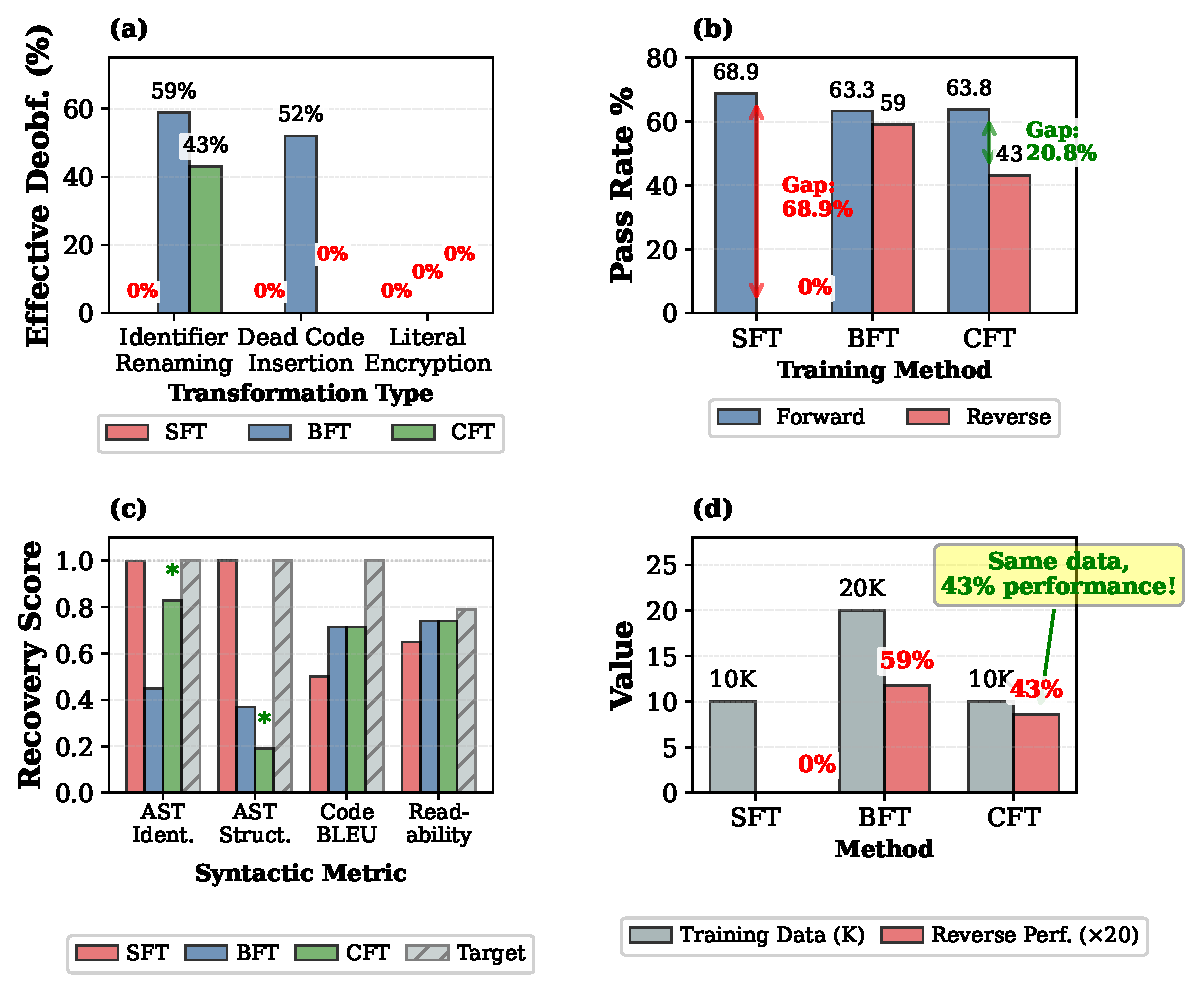
\includegraphics[width=.6\columnwidth, keepaspectratio]{figures/Result_figures/cft_emergent_bidirectionality.pdf}
    \caption{Contrastive fine-tuning partially restores bidirectionality on
    Identifier Renaming but not on the structural or semantic tasks.}
    \label{fig:cft_emergent_bidirectionality}
    \vspace{-0.5cm}
\end{figure}
